
\subsection{Hydrologisk korrigering og konvertering af DTM} \label{Sektion: Konvertering af DTM til DHyM}
Et vigtigt element af en realistisk oversvømmelsesmodellering er at kunne simulere korrekt hydrologisk adfærd gennem terrænet. Dette er nødvendigt at DTM bliver korrigeret og konverteret til en digital hydrologisk terrænmodel (DHyM) for at kunne anvende modellens resultater tillidsfuldt.\\ 

For at konvertere en DTM til en DHyM bliver der anvendt to hydrologiske tilpasningsobjekter: Linje- og hesteskotilpasninger. Begge objekter er linjeobjekter og bliver brændt ned i DTM for at simulere korrekt geografiske karakteristika i landskabet, som ikke er blevet fanget af højdemodellen.\\
Da der findes tilpasninger for både simuleringer af skybrud og stormfloder, er det vigtigt at der kun bliver anvendt de tilpasninger der har indflydelse på havstigning- og stormflodsmodellering. Det betyder derfor at der ikke skal inkluderes tilpasninger, som fx er designet til at føre regnvand fra skybrud ud i havet. Tilpasninger såsom skybrudskontraklappe er derfor blevet fjernet ved at udføre en selektering af de relevante tilpasninger i databasen for hvert område.\\

Dette er gjort for både linje- og hesteskotilpasningerne ved brug af værktøjet \textit{"Extract Hydroconditoning Inundation"}, som foretager en søgning i databaserne for tilpasningslagene. Først søger værktøjet efter alle tilpasninger indenfor områdets afgrænsning. Herefter laves der en søgning i attributtabellen for en anvendelses beskrivelse. Til stormflodsmodellering er der tre relevante attributter og deres funktionalitet er beskrevet i tabel \ref{Tabel: Relevante hydrologiske tilpasninger}. De tilpasninger som opfylder én af kriterierne bliver overført til et nyt lag, en for linjetilpasninger og en for hesteskotilpasninger. 
\begin{table}[H]
\centering
\renewcommand{\arraystretch}{1.5}
\begin{threeparttable}
\caption{Relevante hydrologiske tilpasninger for stormflodsmodellering. Kilde: \cite{GeoDanmark_HydroLag}.}
\label{Tabel: Relevante hydrologiske tilpasninger}
\begin{tabular}{@{} l l @{}} 
\toprule
\textbf{Tilpasningstype} & \textbf{Beskrivelse af tilpasningen} \\
\midrule
\textit{Generel} &
  \makecell[l]{Den normale tilpasning af hydrologiske forhold\\
  (fx skabelse af et frit forløb under en bro)} \\
\addlinespace
\textit{Havstigning} &
  \makecell[l]{Tilpasninger der skal forhindre, at vand løber ind\\
  over det bagvedliggende land\\
  (fx lukning af en højvandssluse)} \\
\addlinespace
\textit{DHMFix} &
  \makecell[l]{Bruges ved ændringer, der har hydrologisk effekt\\
  på vandets frie forløb på terrænoverfladen\\
  (fx reparation af fejl i den specifikke DHM)} \\
\bottomrule
\end{tabular}
\end{threeparttable}
\end{table}
\newpage
Inden tilpasningerne blev brændt ned i DTM, ændres hesteskotilpasningerne fra deres hesteskoform til separate linjer mellem ydersiderne af hesteskoen. Dette gøres for at få den præcise størrelse og udbredelse af tilpasningen brændt ned i DTM fremfor for omridset af tilpasningen. Dette er gjort ved at bruge et Python-script \textit{"Convert Horsehoes to Lines"} hvor både linje- og hesteskotilpasningerne fundet i \textit{"Extract Hydroconditioning Inundation"} bliver omdannet til separate linjer. Konverteringen til separate linjer gør beregningen af højdeværdier i tilpasingen nemmere og dermed nemmere at brænde ned i DTM.\\
De separate linjer til hesteskotilpasningerne blev defineret ud fra de 4 hjørnepunkter af hesteskoen og cellestørrelsen af DTM. Den visuelle ændring af hesteskotilpasningen til linjer er vist i figur \ref{Figur: Ændringen af hesteskotilpasningerne}. Hvor figur \ref{Subfig: Hesteskotilpasninger før ændring} er tilpasningen før ændring og figur \ref{Subfig: Hesteskotilpasning efter tilpasningen er konverteret til linjer} er tilpasningen efter den er blevet konverteret til separate linjer. Hver linje er præcis en cellestørrelse bred (40 cm), da det ikke er nødvendigt med en større linjebredde for at simulere korrekt hydrologisk bevægelse igennem terrænet. 
\begin{figure}[H]
    \begin{subfigure}[t]{0.5\textwidth}
        \centering
        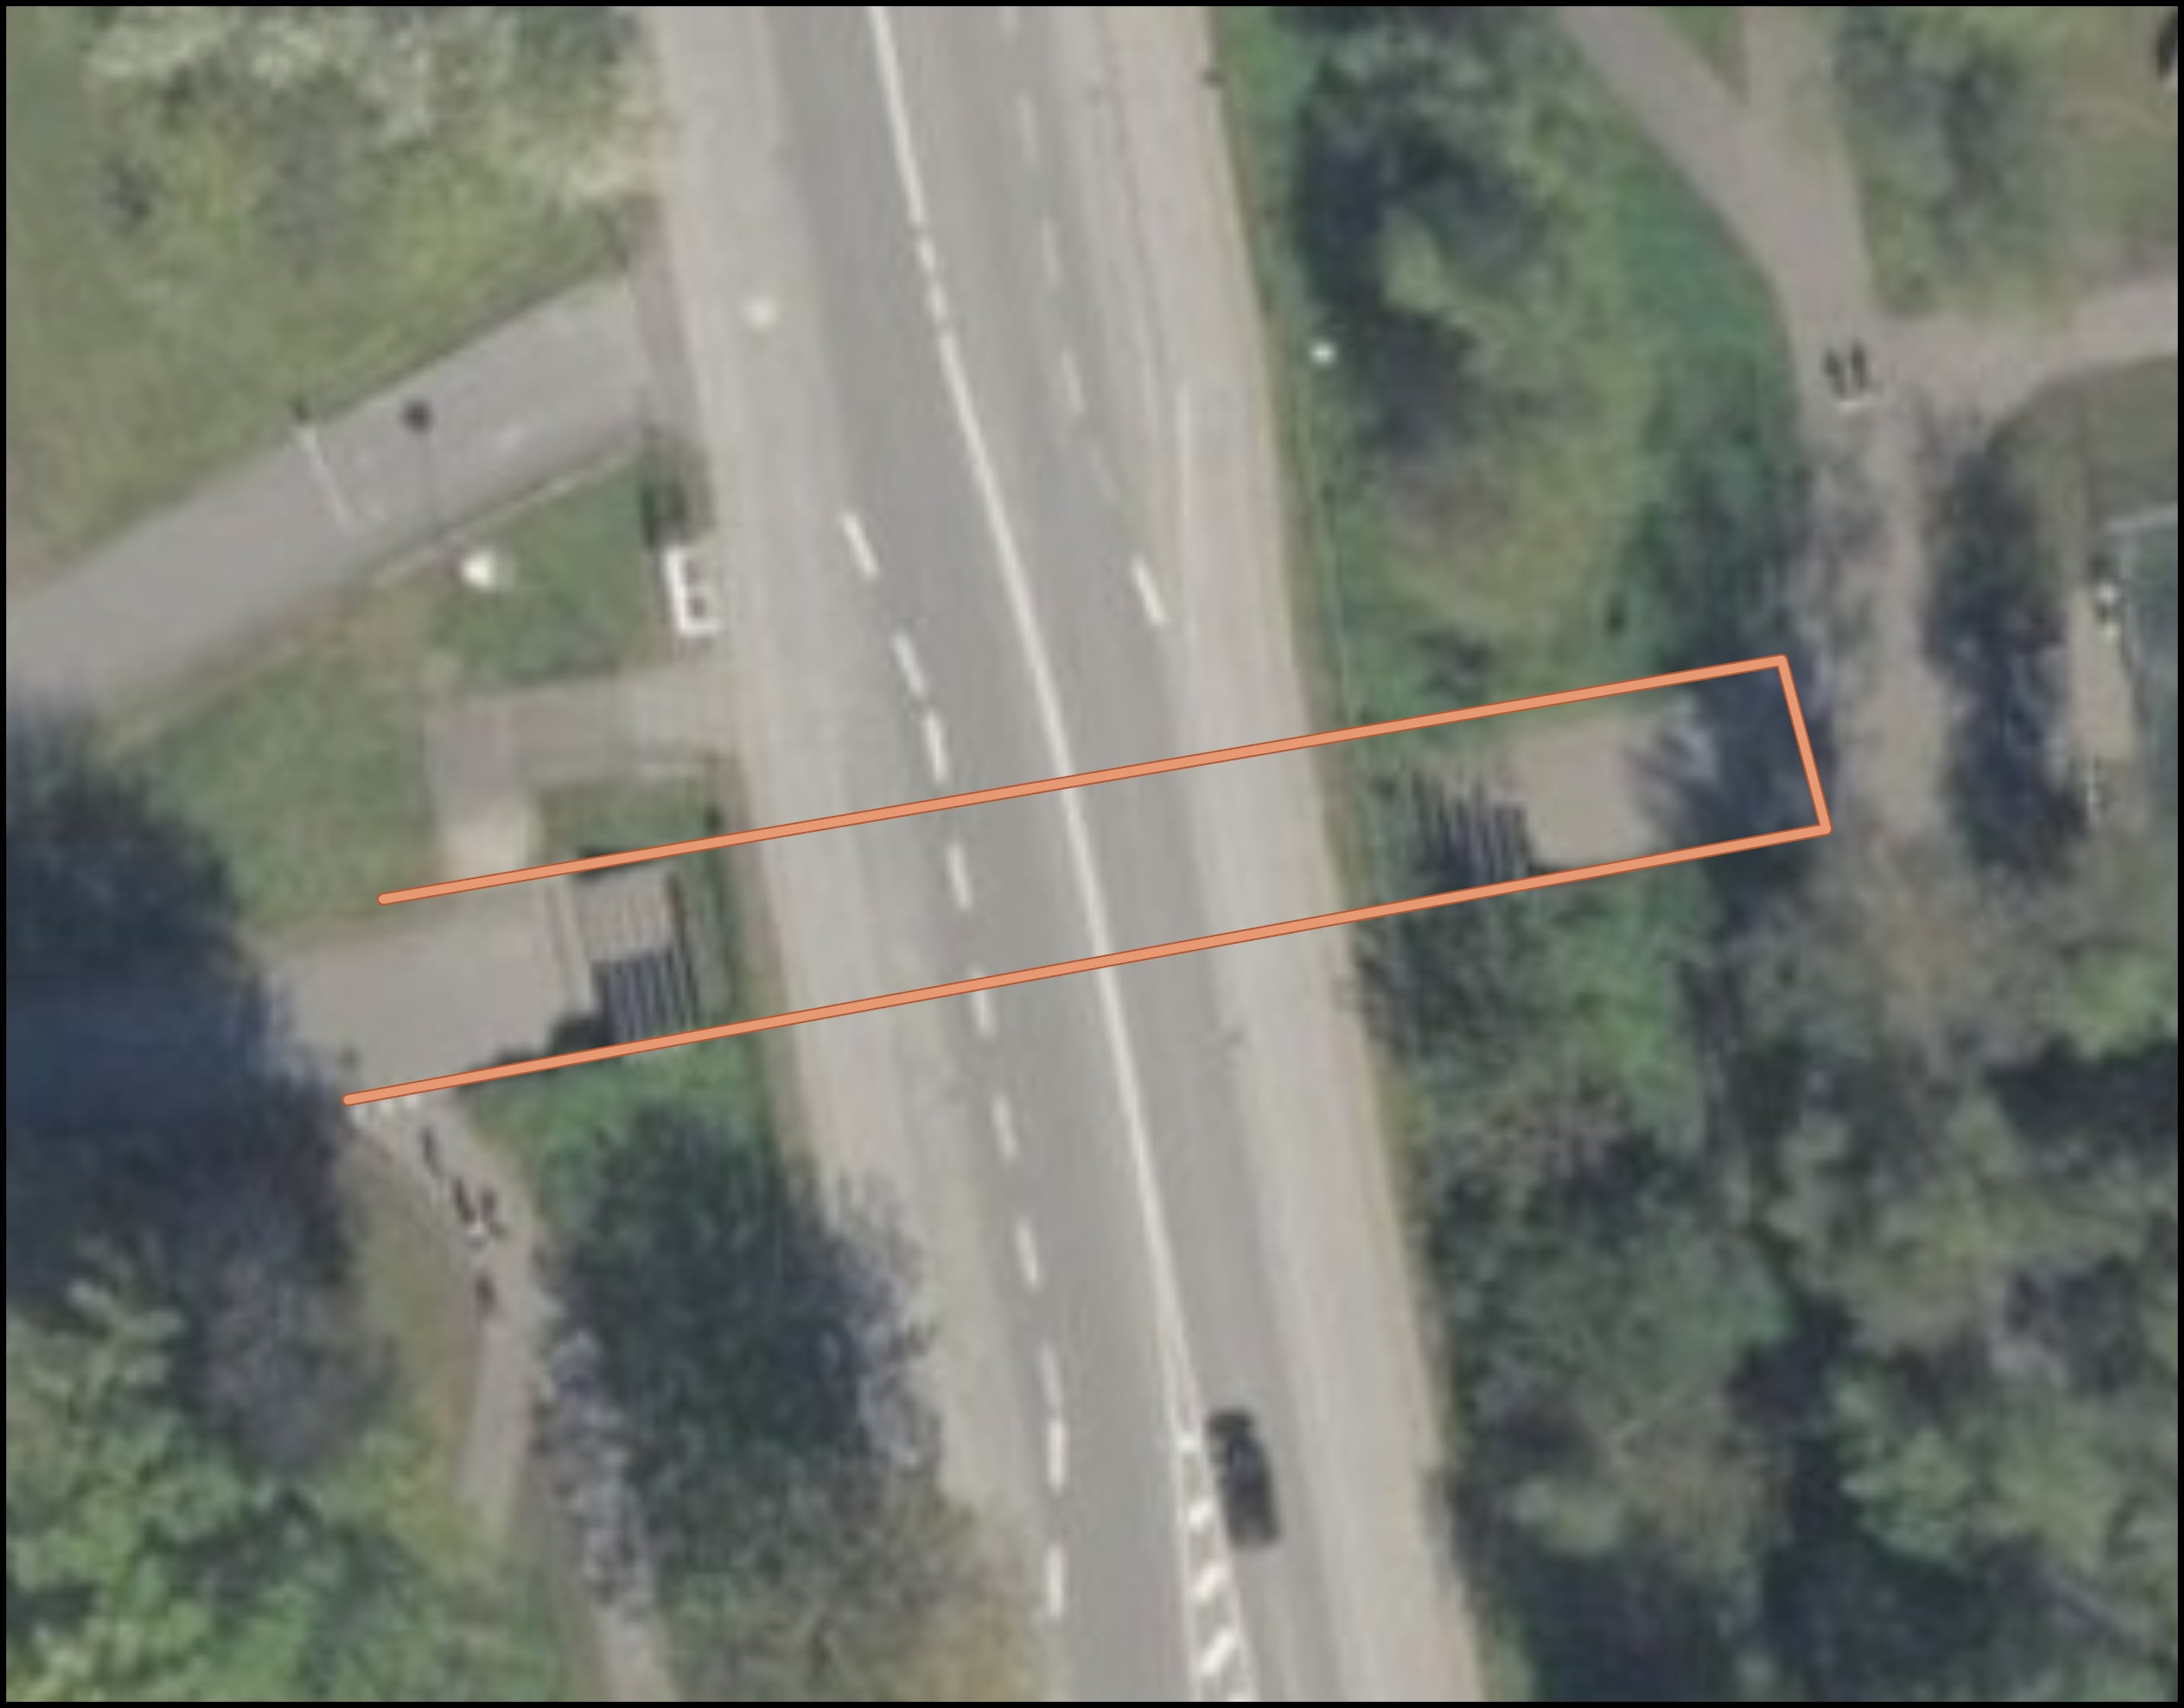
\includegraphics[width=1\linewidth]{images/databeskrivelse/hestesko.jpg}
        \caption{}
        \label{Subfig: Hesteskotilpasninger før ændring}
    \end{subfigure}
    \hspace{0.2cm}
    \begin{subfigure}[t]{0.5\textwidth}
        \centering
        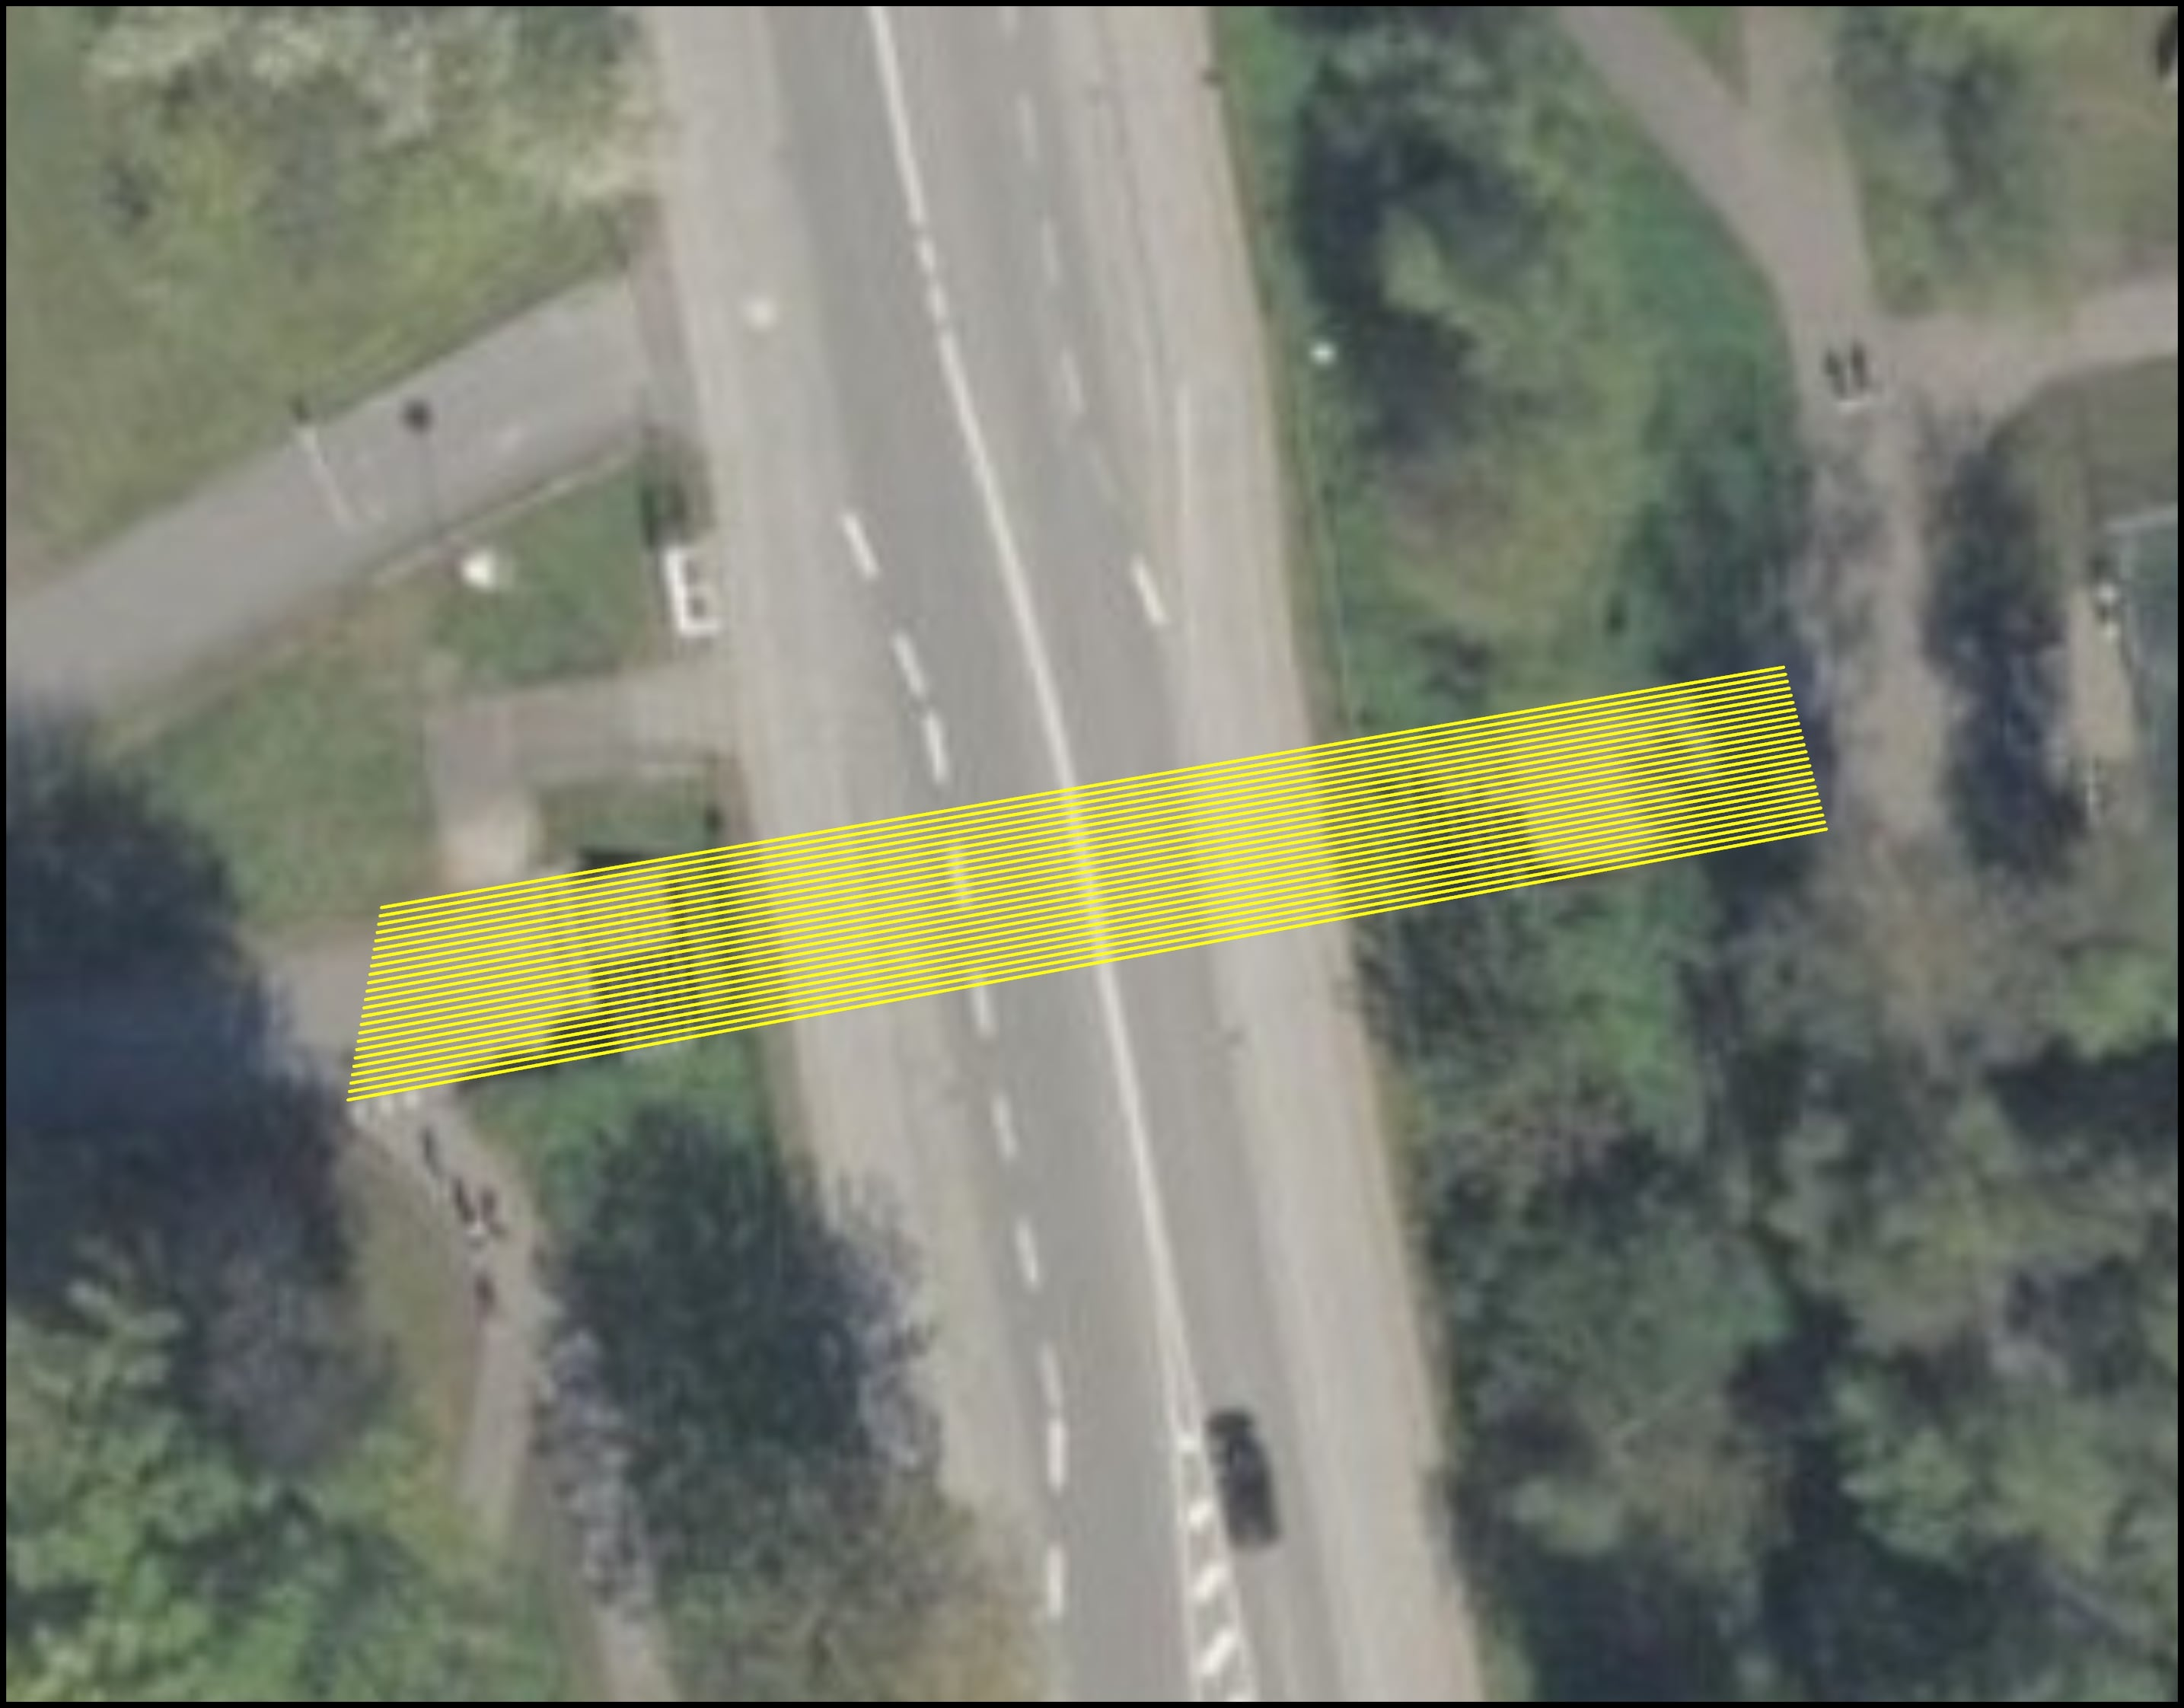
\includegraphics[width=1\linewidth]{images/metode/hestesko_linjer.jpg}
        \caption{}
        \label{Subfig: Hesteskotilpasning efter tilpasningen er konverteret til linjer}
    \end{subfigure}
    \caption{Ændringen af en hesteskotilpasning fra en hesteskoform til separate linjer. \textbf{(a)} Hesteskotilpasningen før ændring. \textbf{(b)} Hesteskotilpasningen efter tilpasningen er konverteret til separate linjer.}
    \label{Figur: Ændringen af hesteskotilpasningerne}
\end{figure}

Dette danner et nyt sammenlagt lag med alle de relevante hydrologiske tilpasninger i et linjeformat. For at tilpasningen bliver korrekt repræsenteret i DHyM skal højdeværdier under terræn hindringer først interpoleres og tildeles til hver tilpasning.\\
Dette blev gjort ved at bruge Python-scriptet \textit{"Hydrologic Conditioning Multiple"} \citep{balstrom_identification_2024}. Scriptet tildeler en z-værdi fra DTM til hver af linjernes endepunkter: $Z_0$ og $Z_1$. Ud fra linjernes endepunkter bliver linjens hældning, $\Delta{Z}$ udregnet ved at bruge afstanden mellem endepunkterne. Linjen konverteres til et rasterformat og derefter til punkter. For hver celle i DTM placeres der et punkt på linjen. Derefter foretages der en lineær interpolation af punkterne langs linjen baseret på startpunktet $Z_0$, afstanden fra $Z_0$ til et punkt og linjens hældning, $\Delta{Z}$. Dette gøres for alle punkter langs linjen (figur \ref{Figur: Interpolation af Z-værdier}). \\

Efter z-værdierne for punkterne er blevet interpoleret, konverteres punkterne tilbage til et rasterformat, hvorefter de hydrologiske tilpasninger brændes ned i DTM ved at kombinere de interpoleret celler i punktrasteren med DTM. Kombineringen sker ved at tjekke for alle celler for NoData værdier i punktrasteren. Hvis værdien er NoData, så anvendes z-værdier fra DTM. Er værdien ikke NoData så erstattes z-værdien i DTM med z-værdien fra punktrasteren.
Samenlagt danner det den korrigeret digitale hydrologiske terrænmodel (DHyM).

\begin{figure}[H]
    \centering
    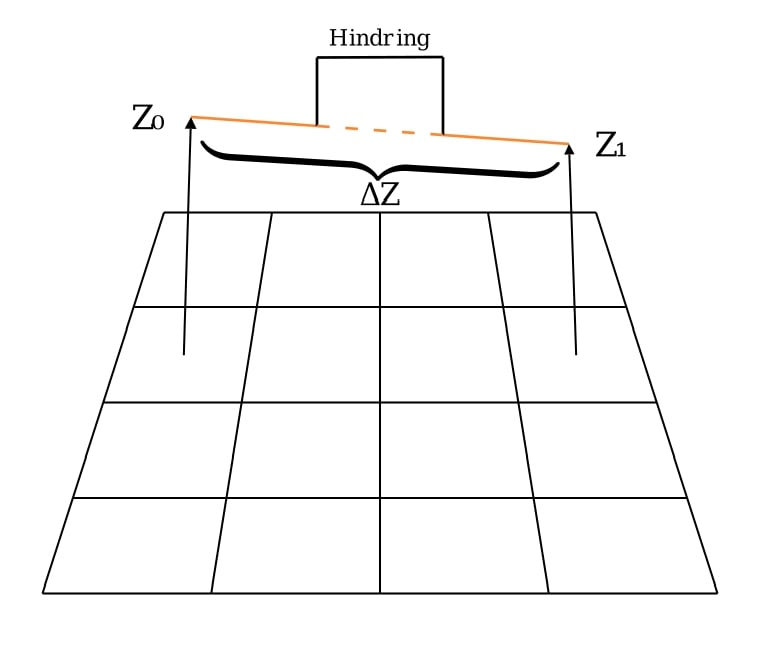
\includegraphics[width=0.5\linewidth]{images/metode/dtm_hydro_z.jpg}
    \caption{Interpolationen af z-værdier langs den orange linje for en linjetilpasning under en hindring. $Z_1$ og $Z_0$ er z-værdierne fra DTM ved linjetilpasningens endepunkter og $\Delta{Z}$ er hældningen af linjetilpasningen. Egen illustration med inspiration fra \cite{balstrom_identification_2024}.}
    \label{Figur: Interpolation af Z-værdier}
\end{figure}

For Aabenraa, Gedser Havn, Hesnæs og Præstø blev der identificeret henholdsvis 250, 13, 34 og 19 relevante hydrologiske tilpasninger, som blev brændt ned i deres tilhørende DTM.


\subsubsection{Inkluderingen af bygninger i DHyM} \label{Afsnit: Inklusion af bygninger i DHyM}

Efter de hydrologiske tilpasninger blev brændt ned i DTM og en DHyM var etableret, blev det besluttet at inkludere bygninger i DHyM, som uigennemtrængelige barrierer i terrænet. Denne beslutning blev truffet med udgangspunkt i, at de oversvømmelseskort leveret fra kommunerne, behandlede bygninger som barrierer. Desuden blev det vurderet at en realistisk simulering af hydrologisk adfærd forudsætter, at vand ikke kan strømme direkte igennem bygninger, men ledes udenom. \\

Metoden for at implementere bygninger i DHyM blev gennemført ved brug af \textit{"Building Block (BB)"} metoden anvendt i \cite{khosh_bin_ghomash_technical_2024}. Metoden hæver terrænhøjden i højdemodellen for hver bygningspolygoners fodaftryk til en bestemt højde. Denne højde blev arbitrært sat til 20 meter for alle bygningerne. Herefter blev bygningspolygonerne konverteret til et rasterformat med den samme cellestørrelse på 40\times40 cm som DHyM. \\
Derefter udføres der et tjek på den nye bygningsraster, hvor celler med en højdeværdi på 20 forblev 20 og celler med NoData blev tildelt værdien 0. Dette sikrer at bygningsrasteren kan kombineres med DHyM, da aritmetiske operationer på NoData-værdier ikke er muligt. Til sidst blev bygningsrasteren og DHyM lagt sammen, hvilket skabte den endelige DHyM, som anvendes i Inundation Modellen.


\subsection{Simulering af 2023-stormfloden}\label{Afsnit: Simulering af stormflod 2023}

Med en DHyM er det muligt at lave stormflodsmodelleringen ved brug af Inundation Modellen. I modellen inputtes der for hvert område den tilhørende DHyM og kildelinjen \textit{"Line at Sea"}. Line At Sea linjen er manuelt digitaliseret et tilfældigt sted i havet for hvert område.\\ 
Hvert område simuleres op til det højeste officielle vandstandsniveau målt under 2023-stormfloden og antallet af iterationer for at opnå dette niveau er vist i tabel \ref{Tabel: Antal iterationer og slutværdier for Inundation Model}. Alle områder starter oversvømmelsessimuleringen med en  starværdi (InitialSeaLevel) på  100 cm og en stigningsværdi (SeaLevelIncrement) på 1 cm. En startværdi på 100 cm blev valgt primært til at minimere processeringstid og stiningsværdien på 1 cm blev valgt for at opnå størst fleksibilitet og gjorde det muligt at opnå nøjagtig samme vandstandsniveau, som målt under stormfloden. Simuleringstiden for hver af de fire områder er vist i tabel \ref{Tabel: Antal iterationer og slutværdier for Inundation Model} og sammenlagt tog det 12 timer og 1 minut at simulere 2023-stormfloden ved for de fire områder på en Lenovo i5-6500T CPU med fire kerner og processorer og 16GB RAM.\\
\begin{table}[H]
\centering
\renewcommand{\arraystretch}{1}
\begin{threeparttable}
\caption{Antal iterationer, slutværdien og processeringstiden for oversvømmelsessimuleringer i Inundation Modellen for simulere oktober 2023 stormfloden.}
\begin{tabular}{@{} l 
                S[table-format=7.2, output-decimal-marker={,}] 
                S[table-format=7.2, output-decimal-marker={,}]
                l @{}} 
\toprule
\textbf{Lokalitet} & \textbf{Antal iterationer} & \textbf{Slutværdi (cm)}  & \textbf{Simuleringstid}\\
\midrule
Aabenraa & 117 & 216 & 5 timer 27 minutter \\
Gedser & 90 & 189 & 3 timer 25 minutter\\ 
Hesnæs & 111 & 210 & 1 time 23 minutter \\
Præstø & 101 & 200 & 1 time 44 minutter \\
\bottomrule
\end{tabular}
\label{Tabel: Antal iterationer og slutværdier for Inundation Model}
\end{threeparttable}
\end{table}

Efter simulgeringen er færdig er der blevet produceret en raster for hver centimeter fra startværdien på 100 til slutværdien. Hver inundationraster viser de celler der oversvømmes ved en bestemt vandstand. Herefter blev der brugt et intern ArcGIS Pro værktøj \textit{"Cell Statistics"} til at finde den minimums vandstand for alle celler i alle rasterlag og kombinere dem sammen til en samlet raster. Denne raster blev filtreret med en landpolygon, så det kun er oversvømmelse på land der bliver medtaget i det endelige resultat af simuleringen. Dette gøres fordi modellen teknisk set simulerer en oversvømmelse på havet mellem Line At Sea-linjen og kysten. Ved at bruge landpolygonen fjernes de ekstra unødvendige værdier fra resultatet.\\
Dette gøres for alle fire områder og producerer dermed de fire simulerede oversvømmelseskort over 2023-stormfloden der kan sammenlignes med de kort hver kommune leverede over vandets udbredelse observeret under stormfloden.  


\subsection{Kvantificering af påvirkede areal anvendelser} \label{Afsnit: Udregning af påvirkede areal anvendelser}

For at kvantificere stormfloden i 2023s påvirkning af studieområderne blev der gennemført en krydstabulering mellem BaseMap04-arealanvendelsekortet og de observerede samt simulerede oversvømmelser af stormfloden.\\

Indledningsvis blev BaseMap04-arealanvendelsesrasteren, med en oprindelige cellestørrelse på 10\times10 meter, resamplet til en cellestørrelse svarende til outputtet fra Inundation Modellen (40\times40 cm). Herefter blev ArcGIS Pro-værktøjet \textit{"Tabulate Area"} anvendt til at kvantificere det oversvømmede areal for hver arealanvendelsesklasse, for både observerede data og modellens resultater.
 
\begin{figure}[H]
    \centering
    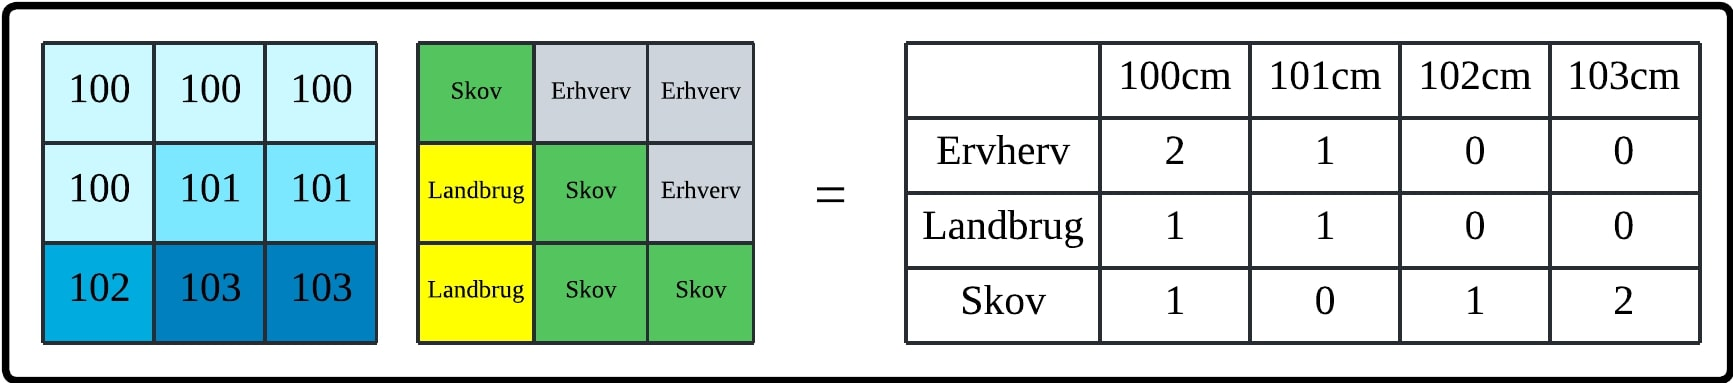
\includegraphics[width=1\linewidth]{images/metode/tabulate.jpg}
    \caption{Krydstabulerings processen bag Tabulate Area værktøjet i ArcGIS Pro. Hver celle i oversvømmelsesrasteren kobles til en celle i arealanvendelsesrasteren og tabuleres. Egen illustration med inspiration fra \cite{esri_tabulate_nodate}.}
    \label{Figur: Tabulate}
\end{figure}
Værtøjet Tabulate Area krydsreferer hver celle i BaseMap-arealanvendelsesrasteren med den tilsvarende celle i oversvømmelsesrasteren, således at der knyttes en specifik arealanvendelse til et givent oversvømmelsesniveau. Dette muliggør en kvantitativ vurdering af stormflodens påvirkning på forskellige arealanvendelser i studieområderne (figur \ref{Figur: Tabulate}).\\

Resultatet af krydstabuleringen præsenteres i form af en kontingenstabel, hvor rækkerne repræsenterer de forskellige arealanvendelsesklasser, og kolonner angiver de respektive oversvømmelsesnivauer i centimeter. Ud fra denne tabel summeres antallet af celler for hver unik arealanvendelse, hvorefter det samlede oversvømmede areal for her klasse beregnes som en andel af det totale oversvømmede areal. Resultatet visualiseres efterfølgende i form af søjlediagrammer.

\subsection{Statistisk 100-års hændelse og fremskrivningen af 2023-stormfloden} \label{Afsnit: Fremskrivning og statistisk}
I lyset af fremtidige klimaforandringer og risikoen for stigende vandstand i Danmark, undersøges der hvordan hvordan en oversvømmelse vil se ud ved to forskellige stormflodshændelser: et statistisk vandstandsniveau ved en 100-års stormflodshændelse og en fremskrivning af hvordan 2023-stormfloden til 2100 vil se ud baseret på vandstandsprojektioner fra den sjette \cite{ipcc_report_AR6} rapport. For begge hændelsestyper simuleres der for to forskellige Shared Socioeconomic Pathways (SSP) scenarier: et mellemhøjt udledningsscenarie (SSP2-4,5) og et meget højt udledningsscenarie (SSP5-8,5). Det mellemhøje scenarie blev valgt som en kompromisbaseret mellemposition mellem det højeste mulige klimascenarie og det mildeste, selvom \cite{dmi_ny_nodate} understreger, at kommunerne og forvaltningsinteressenter bør bruge det høje scenarie (SSP3-7) i klimavurderinger. Det meget høje scenarie blev valgt for at simulere en stormflod under det værst mulige udfald.\\

{\large \textit{Statistisk 100-års hændelse}}\\
For at undersøge påvirkningen af områderne baseret på en statistisk 100-års hændelse, blev DMIs Klimaatlas anvendt til at bestemme vandstandshøjden af en stormflod der statistisk set vil optræde en gang per 100 år. Klimaatlas inddeler Danmarks kyster i kyststrækninger og de fire kyststrækninger der blev anvendt er: Lillebælt Syd for Aabenraa, Femern Bælt for Gedser, Falsters og Møns Østersøkyst for Hesnæs og Faxe Bugt for Præstø. For hver kyststrækning anvendes den absolute vandstandshøjde for en 100-års hændelse ved SSP2,5-4,5 og SSP5-8,5.\\

Herefter bruges Inundation Modellen til at simulere op til SSP5-8,5 scenariet for hvert område. Processen bag dette er den samme som i afsnit \ref{Afsnit: Simulering af stormflod 2023}, men i stedet for at starte ved 100 cm starter modellen ved den observerede vandstandshøjde ved stormfloden for hvert område. Der blev simuleret op til en vandstandshøjde på 251 cm for Aabenraa, 242 cm for Gedser, 253 cm for Hesnæs og 225 cm for Præstø og tilføjede sammenlagt en ekstra 2 timer og 46 minutter i simuleringstid. \\

{\large \textit{Fremskrivning af 2023-stormfloden}} \\
Da vandstanden i Danmark forventes at stige i løbet af det nuværende århundrede har det derfor været ønsket at undersøge hvordan 2023 stormflodshændelsen vil se ud hvis den skete i slutningen af det nuværende århundrede. Til at gøre dette er der lavet en beregning af middelvandstanden i 2100. DMIs Klimaatlas har allerede værdier for middelvandstanden i 2100, men deres værdier er i forhold til en referenceperiode fra 1981-2010. Det har derfor været nødvendige at beregne middelvandstandsniveauet i 2023 i forhold til DMIs referenceperiode og derefter beregne hvad middelvandstanden vil være i 2100 baseret på vandstanden i 2023.\\ 
\newpage
Til at udføre denne udregning er der blevet anvendt et datasæt fra \cite{garner_ipcc_2021} over havspejlsprojektioner og et online værktøj udviklet af \cite{NASA_tool}. NASAs værktøj gør det muligt at få projektioner til en bestemt Permanent Service for Mean Sea Level (PSMSL) station. I værktøjet vælges den nærmeste PSMSL-station for hvert område. Stationen blev udvalgt ud fra hvilket hav basin, der var tættest på hvert område. Dette var Fynshav for Aabenraa, Gedser Havn for Gedser, Warnemünde for Hesnæs og Skanör for Præstø.\\ 

Værktøjet giver derefter en tabel med alle de individuelle bidrag til havspejlsstigning og en median havspejlsstigning ($SLR_{50}$) for hver station i forhold til en referenceperiode fra 1995-2014. $SLR_{50}$ indeholder en række faktorer der påvirker havspejlsstigning, såsom ferskvandstilførsel fra floder, glacial bidrag og tager højde for lokal isostasi. For at udregne middelvandstanden i 2023, er projektionen for 2030 anvendt, da det er den nærmeste. Til udregningen er der blevet opstillet følgende ligning: 
\begin{align} \label{Equation: Vandstandsstigning calculation}
    S_r = S_p- \left( \frac{\Delta{t}}{\Delta{t_r}}\times SLR_{50} + \Delta{M_r} \times \left(\frac{SLR_{50}}{\Delta{t_r}}\right) \right)
\end{align}
Middelvandstanden i 2023 beregnes ved at finde forholdet af differencen mellem målåret 2023 ($\Delta{t}$), NASAs referenceår ($\Delta{t_r}$) og projektionsåret (2030). Dette forhold ganges med $SLR_{50}$ og giver middelvandstanden i 2023 i forhold til NASAs referenceperiode 1995-2014. Herefter beregnes den forventede middelvandstandsstigning fra DMIs referenceperiode (1981-2010) til NASAs referenceperiode (1995-2014). Denne udregning er lavet under den antagelse at stigningen fra DMIs referenceperiode til NASAs reference har været lineær \citep{danish_meteorological_institute_dmi_2024}. Dette gøres ved at tage differencen mellem referenceperiodernes median år ($\Delta{M_r}$) og gange med raten af havspejlstigning ($\frac{SLR_{50}}{\Delta{t_r}}$) frem mod 2030. \\
Dette giver et resultat for hvad middelvandstanden i 2023 har været i forhold til DMIs referenceperiode og gør det muligt at fratrække denne vandstand fra den projekteret vandstand i 2100 ($S_p$) og giver $S_r$, som er middelvandstanden i 2100 med 2023 som det nye referenceår. Denne fremgangsmåde blev udført ved et SSP2-4,5 og et SSP5-8,5 scenarie.\\

Herefter blev Inundation Modellen igen kørt for at få nye oversvømmelsesdata. Der blev simuleret op til 268 cm for Aabenraa, 259 for Hesnæs og 246 for Præstø. Der blev ikke simuleret en ny stormflod for Gedser da 100-års hændelsen ved SSP8.5 er en højere vandstand end den fremskrevet stormflod i 2100. Fremskrivningen tilføjede en yderlig 1 time og 58 minutter til samlet simuleringstid.\\

Derefter blev alle oversvømmelsesrasterne konverteret til polygoner og kombineret med værktøjet \textit{"Merge"} for at få visualiseret oversvømmelser fra en 100-års hændelse og en fremskrivning af stormfloden på et samlet kort.